\documentclass{article}



\usepackage[framed,numbered,autolinebreaks,useliterate]{mcode}
\usepackage{graphicx}
\usepackage{float}

\setlength{\parindent}{0pt}
\setlength{\parskip}{18pt}
\title{\texttt{Predator Vs Prey Simulation}}
\author{Matthew Ginelli}
\date{April 2012}




\begin{document}

\maketitle

\textbf{NOTE}

The attached code, \texttt{examplecode.m} runs the three methods to produce a 2x1 subplot to include the Euler'sapproximation of each population along with the ode45~approximation and the second is to include the Runge-Kutta approximation with the ode45 approximation.

\medskip

\textbf{Code}

\lstinputlisting{examplecode.m}
\textbf{Figures}

Below are the outputs from the simulations

\begin{figure}[ht]
\centering
    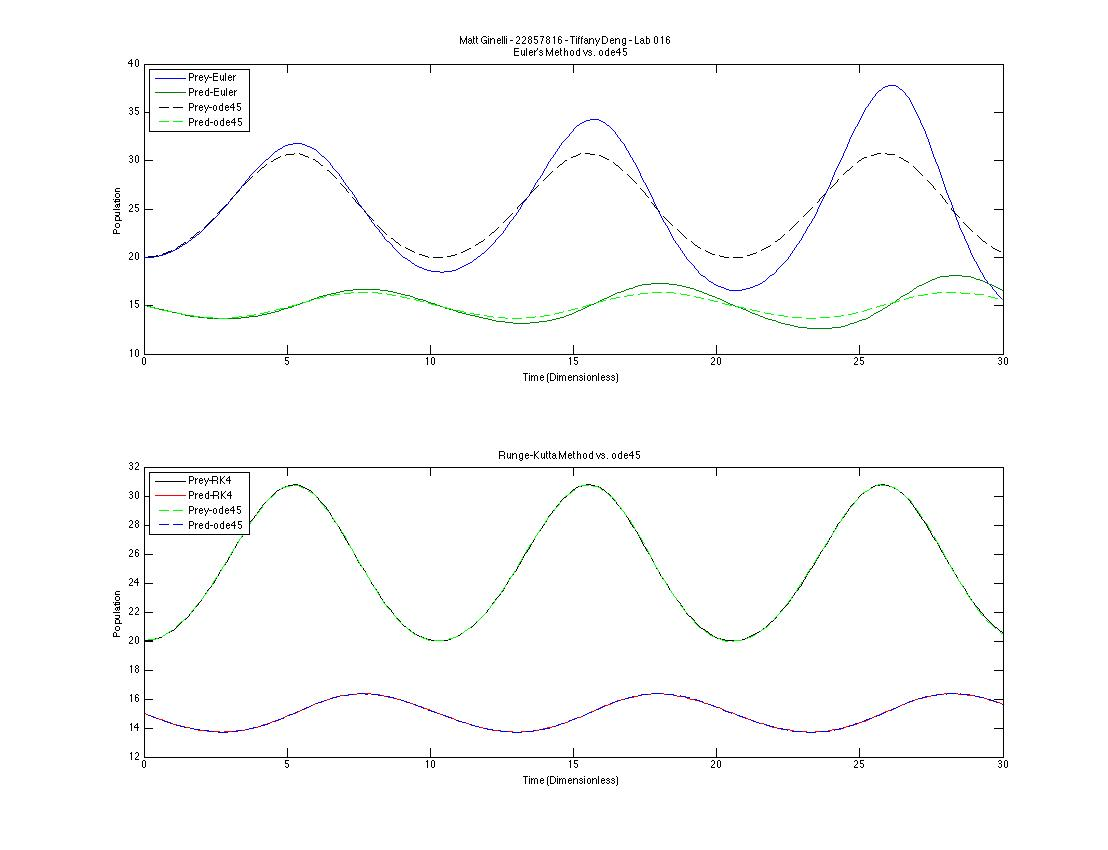
\includegraphics[width=\textwidth,height=\textheight,keepaspectratio]{example.jpg}%
    \caption{Simulator Results}
    \label{fig:example}
\end{figure}


Matthew F. Gienlli (\texttt{matt.uhs@gmail.com})

\end{document}